\documentclass[a4paper, 11pt]{article}

% ====== PACCHETTI NECESSARI ======
\usepackage[utf8]{inputenc}
\usepackage[T1]{fontenc}
\usepackage[italian]{babel}
\usepackage{geometry}
\usepackage{graphicx}
\usepackage[table]{xcolor}
\usepackage{tabularx}
\usepackage{array}
\usepackage{amssymb}
\usepackage{fancyhdr}
\usepackage{titlesec}
\usepackage{helvet}
\renewcommand{\familydefault}{\sfdefault}
\usepackage{lipsum}
\usepackage{hyperref}
\usepackage{booktabs}
\usepackage{enumitem}
\usepackage{tcolorbox}
\usepackage{amsmath}
\usepackage{longtable}
\usepackage{float}

% ====== IMPOSTAZIONI GLOBALI DI STILE ======

% 1. DEFINIZIONE COLORI BLU-VIOLA
\definecolor{AccentColor}{RGB}{80, 90, 180}
\definecolor{AccentLight}{RGB}{80, 90, 180}
\definecolor{AccentDark}{RGB}{50, 60, 140}
\definecolor{LightGray}{RGB}{245, 245, 250}
\definecolor{MediumGray}{RGB}{200, 200, 210}
\definecolor{WarnBg}{RGB}{253, 236, 234}
\definecolor{WarnBorder}{RGB}{192, 57, 43}
\definecolor{InfoBg}{RGB}{237, 232, 251}

% 2. IMPOSTAZIONE MARGINI
\geometry{a4paper, left=2.5cm, right=2.5cm, top=3.5cm, bottom=3.5cm}

% 3. STILE DEI TITOLI DI SEZIONE
\titleformat{\section}
{\normalfont\sffamily\Large\bfseries\color{AccentColor}}
{\thesection}
{1em}
{}
\titleformat{\subsection}
{\normalfont\sffamily\large\bfseries\color{AccentDark}}
{\thesubsection}
{1em}
{}
\titleformat{\subsubsection}
{\normalfont\sffamily\large\bfseries\color{AccentDark}}
{\thesubsubsection}
{1em}
{}
\titleformat{\paragraph}
{\normalfont\sffamily\large\bfseries\color{AccentDark}}
{\theparagraph}
{1em}
{}

% ====== GESTIONE GERARCHIA TITOLI ======

% ==========================================
% DEFINIZIONE LIVELLO 4: \subsubsubsection
% ==========================================
\titleclass{\subsubsubsection}{straight}[\subsubsection]
\newcounter{subsubsubsection}[subsubsection]
\renewcommand{\thesubsubsubsection}{\thesubsubsection.\arabic{subsubsubsection}}

\titleformat{\subsubsubsection}
  {\normalfont\normalsize\bfseries}
  {\thesubsubsubsection}{1em}{}

\titlespacing*{\subsubsubsection}
  {0pt}{3.25ex plus 1ex minus .2ex}{1.5ex plus .2ex}

% ==========================================
% DEFINIZIONE LIVELLO 5: \subsubsubsubsection
% ==========================================
\titleclass{\subsubsubsubsection}{straight}[\subsubsubsection]
\newcounter{subsubsubsubsection}[subsubsubsection]
\renewcommand{\thesubsubsubsubsection}{\thesubsubsubsection.\arabic{subsubsubsubsection}}

\titleformat{\subsubsubsubsection}
  {\normalfont\normalsize\bfseries\itshape}
  {\thesubsubsubsubsection}{1em}{}

\titlespacing*{\subsubsubsubsection}
  {0pt}{3.25ex plus 1ex minus .2ex}{1.5ex plus .2ex}

% ==========================================
% GESTIONE INDICE (TOC) E NUMERAZIONE
% ==========================================

\setcounter{secnumdepth}{5}
\setcounter{tocdepth}{5}

% Formattazione per Livello 4
\titleformat{\subsubsubsection}
  {\normalfont\sffamily\large\bfseries\color{AccentDark}}
  {\thesubsubsubsection}
  {1em}
  {}

% Formattazione per Livello 5
\titleformat{\subsubsubsubsection}
  {\normalfont\sffamily\large\bfseries\color{AccentDark}}
  {\thesubsubsubsubsection}
  {1em}
  {}

% ====== IMPOSTAZIONE HEADER E FOOTER ======
\pagestyle{fancy}
\fancyhf{}
\fancyhead[L]{\sffamily\bfseries\color{AccentColor}BYTE HOLDERS}
\fancyhead[R]{\sffamily\color{AccentColor}\thepage}
\renewcommand{\headrulewidth}{0.8pt}
\renewcommand{\headrule}{\color{AccentColor}\hrule width\headwidth height\headrulewidth \vskip-\headrulewidth}

% ====== IMPOSTAZIONE LINK ======
\hypersetup{
  colorlinks=true,
  linkcolor=AccentColor,
  urlcolor=AccentLight,
  citecolor=AccentDark,
}

% ====== PERSONALIZZAZIONE ELENCHI ======
\setlist[itemize]{itemsep=2pt, topsep=4pt}
\setlist[enumerate]{itemsep=2pt, topsep=4pt}

% ====== COMANDI PERSONALIZZATI ======
\makeatletter
\newcommand{\NomeGruppo}[1]{\def\@NomeGruppo{#1}}
\newcommand{\TitoloVerbale}[1]{\def\@TitoloVerbale{#1}}
\newcommand{\Sommario}[1]{\def\@Sommario{#1}}
\newcommand{\Autore}[1]{\def\@Autore{#1}}
\newcommand{\Verificatore}[1]{\def\@Verificatore{#1}}
\makeatother
\newcommand{\lastVisited}[3]{\textit{(Visitato: #1/#2/#3)}}

% ====== STILE TABELLE MIGLIORATO ======
\newcolumntype{Y}{>{\raggedright\arraybackslash}X}
\setlength{\arrayrulewidth}{0.4pt}
\setlength{\tabcolsep}{10pt}
\renewcommand{\arraystretch}{1.4}

% ====== BOX DI AVVISO ======
\newtcolorbox{warnbox}{
  colback=WarnBg,
  colframe=WarnBorder,
  boxrule=0.6pt,
  arc=3pt,
  left=8pt, right=8pt, top=6pt, bottom=6pt
}

\newtcolorbox{infobox}{
  colback=InfoBg,
  colframe=AccentColor,
  boxrule=0.6pt,
  arc=3pt,
  left=8pt, right=8pt, top=6pt, bottom=6pt
}

\newtcolorbox{rolebox}[1]{
  colback=LightGray,
  colframe=AccentDark,
  boxrule=0.6pt,
  arc=3pt,
  left=8pt, right=8pt, top=6pt, bottom=6pt,
  title=\textbf{Ruolo richiesto: #1}
}

% ====== INIZIO DEL DOCUMENTO ======
\makeatletter
\def\toclevel@subsubsubsection{4}
\def\toclevel@subsubsubsubsection{5}
\def\toclevel@paragraph{6}
\def\toclevel@subparagraph{7}
\renewcommand\l@section{\@dottedtocline{1}{0em}{3em}}
\renewcommand\l@subsection{\@dottedtocline{2}{3em}{3.8em}}
\renewcommand\l@subsubsection{\@dottedtocline{3}{6.8em}{4.6em}}
\def\l@subsubsubsection{\@dottedtocline{4}{7em}{4.1em}}
\def\l@subsubsubsubsection{\@dottedtocline{5}{11em}{5em}}
\let\l@paragraph\@gobbletwo
\let\l@subparagraph\@gobbletwo
\makeatother

\begin{document}
% ====== INFORMAZIONI PER LA PAGINA DI TITOLO ======

\makeatletter
\def\toclevel@paragraph{6}
\def\toclevel@subparagraph{7}
\makeatother

\NomeGruppo{BYTE HOLDERS}
\TitoloVerbale{Manuale Utente\textsuperscript{G}}
\Autore{}
\Verificatore{}

\pagestyle{empty}

% ====== PAGINA DI TITOLO ======
\begin{titlepage}
  \centering

  
\includegraphics[width=0.55\textwidth]{../Assets/ByteHolders1.png}\par\vspace{1.5cm}
  \begin{figure}
    \centering
    \label{fig:placeholder}
  \end{figure}

  {\LARGE \sffamily \color{AccentColor}\bfseries Manuale Utente}\par
  \vspace{0.5cm}
  {\large \color{AccentColor}\sffamily }\par

  \vfill

  \noindent\color{AccentColor}\rule{\textwidth}{1pt}\par
  \vspace{0.5cm}

  \begin{tabularx}{0.9\textwidth}{@{}>{\bfseries\sffamily}l X@{}}
    Autore & \sffamily Alessandro Morabito, Alessandro Frison, Lorenzo Grolla, Nicolò Lattanzio, Damiano Berti, Giacomo Nalotto, Giulia Romanato\\
    \arrayrulecolor{MediumGray}\hline \\[-1.5ex]
    Verificatore & \sffamily Alessandro Morabito, Alessandro Frison, Lorenzo Grolla, Nicolò Lattanzio, Damiano Berti, Giacomo Nalotto\\
    \arrayrulecolor{MediumGray}\hline \\[-1.5ex]
    Approvazione & Alessandro Morabito\sffamily \\
    \arrayrulecolor{MediumGray}\hline
  \end{tabularx}
c
  \vfill
\end{titlepage}

\newpage
\section*{Registro delle versioni}

\rowcolors{2}{LightGray}{white}
\begin{longtable}{>{\centering\arraybackslash}p{1.35cm} >{\centering\arraybackslash}p{1.8cm} >{\raggedright\arraybackslash}p{2.1cm} >{\raggedright\arraybackslash}p{2.1cm} >{\raggedright\arraybackslash}p{5cm}}
  % --- Intestazione per la PRIMA pagina ---
  \rowcolor{AccentColor}
  \textcolor{white}{\textbf{Versione}} &
  \textcolor{white}{\textbf{Data}} &
  \multicolumn{1}{c}{\textcolor{white}{\textbf{Autore}}} &
  \multicolumn{1}{c}{\textcolor{white}{\textbf{Verificatore}}} &
  \multicolumn{1}{c}{\textcolor{white}{\textbf{Descrizione delle modifiche}}} \\
  \endfirsthead

  % --- Intestazione per le Pagine SUCCESSIVE ---
  \rowcolor{AccentColor}
  \textcolor{white}{\textbf{Versione}} &
  \textcolor{white}{\textbf{Data}} &
  \multicolumn{1}{c}{\textcolor{white}{\textbf{Autore}}} &
  \multicolumn{1}{c}{\textcolor{white}{\textbf{Verificatore}}} &
  \multicolumn{1}{c}{\textcolor{white}{\textbf{Descrizione (continua)}}} \\
  \endhead

  % --- Dati della tabella ---
  1.0.0 & 25/04/2026 & Giacomo Nalotto & Alessandro Morabito & Approvazione finale del documento\\
  0.6.0 & 24/04/2026 & Nicolò Lattanzio & Damiano Berti & Aggiunta immagini interfaccia utente \\
  0.5.0 & 23/04/2026 & Giulia Romanato & Damiano Berti & Aggiunta sezione Risoluzione dei problemi e Glossario \\
  0.4.0 & 22/04/2026 & Lorenzo Grolla & Alessandro Frison & Aggiunta sezione Visualizzazione del report \\
  0.3.0 & 22/04/2026 & Alessandro Morabito & Nicolò Lattanzio & Aggiunte sezioni Gestione repository ed Esecuzione scansione \\
  0.2.0 & 21/04/2026 & Damiano Berti & Giacomo Nalotto & Aggiunte sezioni Gestione workspace e Gestione membri \\
  0.1.0 & 20/04/2026 & Alessandro Frison & Lorenzo Grolla & Creazione documento, Introduzione e Requisiti di sistema \\
\end{longtable}
\newpage

% ====== INDICE ======
\pagestyle{fancy}
\newpage
\tableofcontents
\newpage
\listoffigures
\newpage
\listoftables
\newpage

% =====================================================================
% ====== SEZIONE INFORMAZIONI INTRODUTTIVE ======
% =====================================================================

\section{Introduzione}

\subsection{Scopo del documento}
Il presente documento si pone l'obiettivo di guidare l'utente all'uso della piattaforma \textbf{CodeGuardian}, fornendo una descrizione esaustiva delle funzionalità offerte e delle procedure operative necessarie per sfruttarle al meglio. Il manuale rappresenta il riferimento principale a cui gli utenti finali possono rivolgersi in caso di dubbi sull'utilizzo del software o in presenza di situazioni non previste durante la normale interazione con la piattaforma.

Il documento copre l'intero ciclo d'uso dell'applicativo, dall'autenticazione iniziale fino alla consultazione dei report di analisi, ed è strutturato in modo da supportare tutti i ruoli previsti dal sistema.

Nello specifico, questo documento si propone di:
\begin{itemize}
  \item \textbf{Indicare i requisiti di sistema}: elencando i browser e le condizioni di rete necessari al corretto funzionamento dell'applicativo;
  \item \textbf{Descrivere il flusso di autenticazione}: illustrando la procedura di accesso tramite Amazon Cognito\textsuperscript{G} e la gestione delle sessioni\textsuperscript{G};
  \item \textbf{Presentare le funzionalità disponibili}: documentando, per ogni ruolo utente, le operazioni eseguibili su workspace\textsuperscript{G}, repository\textsuperscript{G}, scansioni\textsuperscript{G} e report\textsuperscript{G};
  \item \textbf{Fornire procedure operative dettagliate}: guidando l'utente passo-passo attraverso le principali attività;
  \item \textbf{Trattare le casistiche di errore}: elencando le situazioni anomale più frequenti con relative diagnosi e soluzioni.
\end{itemize}

\subsection{Glossario}
Al fine di prevenire ambiguità e garantire una comunicazione uniforme e precisa tra i membri del gruppo e i committenti, è stato redatto un Glossario\textsuperscript{G} apposito.
Per facilitare la lettura del presente documento, i termini tecnici o dotati di un significato specifico all'interno del dominio di progetto sono contrassegnati da una lettera «G» posta in apice (es. Parola\textsuperscript{G}), e la loro spiegazione consultata nella sezione \ref{sec:glossario}.

\subsection{Scopo del prodotto}
Il sistema CodeGuardian è progettato per condurre analisi approfondite sulla qualità di repository GitHub\textsuperscript{G}, garantendo un controllo rigoroso sulla gestione degli accessi e sull'autorizzazione all'avvio delle procedure di scansione\textsuperscript{G}. Dal punto di vista dell'utente finale, la piattaforma si presenta come un'applicazione web che permette di:
\begin{itemize}
    \item organizzare i repository all'interno di ambienti collaborativi (i workspace\textsuperscript{G}), condivisi fra più utenti;
    \item invitare altri utenti a collaborare, assegnando loro ruoli con differenti livelli di autorizzazione;
    \item avviare scansioni su specifici branch\textsuperscript{G} di un repository;
    \item consultare i report\textsuperscript{G} prodotti dagli agenti di intelligenza artificiale, suddivisi in sezioni dedicate a tecnologie, test, sicurezza e documentazione.
\end{itemize}

\subsection{Destinatari del documento}
Il presente manuale è rivolto a tutti gli utenti della piattaforma, indipendentemente dal loro ruolo. La descrizione delle funzionalità tiene conto delle differenze di autorizzazione previste per i tre ruoli supportati:
\begin{itemize}
    \item \textbf{Project Manager}\textsuperscript{G};
    \item \textbf{Tech Lead}\textsuperscript{G};
    \item \textbf{Developer}\textsuperscript{G}.
\end{itemize}
Le sezioni o le operazioni riservate a uno specifico ruolo sono evidenziate da un apposito riquadro che ne indica l'autorizzazione richiesta.

\subsection{Riferimenti}

\subsubsection{Riferimenti normativi}
\begin{itemize}
  \item
    Norme Di Progetto\textsuperscript{G} V2.0.0\\
    \url{https://byte-holders.github.io/Documentazione/PB/Norme_Di_Progetto-V2.0.0.pdf}
  \item
    Capitolato\\
    \url{https://www.math.unipd.it/~tullio/IS-1/2025/Progetto/C2.pdf}\\
    \lastVisited{29}{04}{2026}
\end{itemize}

\subsubsection{Riferimenti informativi}
\begin{itemize}
  \item
    GitHub Docs -- About repositories\\
    \url{https://docs.github.com/en/repositories/creating-and-managing-repositories/about-repositories}\\
    \lastVisited{29}{04}{2026}
  \item
    GitHub Docs -- Managing your personal access tokens\\
    \url{https://docs.github.com/en/authentication/keeping-your-account-and-data-secure/managing-your-personal-access-tokens}\\
    \lastVisited{29}{04}{2026}
  \item
    OWASP Top 10\\
    \url{https://owasp.org/www-project-top-ten/}\\
    \lastVisited{29}{04}{2026}
  \item
  	CVE -- Common Vulnerabilities and Exposures\\
  	\url{https://www.cve.org/}\\
  	\lastVisited{29}{04}{2026}
  \item
    CWE -- Common Weakness Enumeration\\
    \url{https://cwe.mitre.org/}\\
    \lastVisited{29}{04}{2026}
\end{itemize}

\newpage
% =====================================================================
\section{Requisiti di sistema}
% =====================================================================

Questa sezione elenca i requisiti hardware e software necessari al corretto funzionamento dell'applicativo web CodeGuardian.

\subsection{Browser supportati}

Il corretto funzionamento dell'applicativo web è garantito sui sistemi desktop equipaggiati con sistemi operativi che supportano i seguenti browser:

\begin{table}[H]
\centering
\rowcolors{2}{LightGray}{white}
\begin{tabular}{>{\raggedright\arraybackslash}p{5cm} >{\raggedright\arraybackslash}p{6cm}}
\rowcolor{AccentColor}
\textcolor{white}{\textbf{Browser}} & \textcolor{white}{\textbf{Versione minima}} \\
Google Chrome    & v. 120 o superiore \\
Mozilla Firefox  & v. 121 o superiore \\
Microsoft Edge   & v. 120 o superiore \\
Apple Safari     & v. 17 o superiore  \\
Opera            & v. 105 o superiore  \\

\end{tabular}
\caption{Compatibilità browser}
\label{tab:browser}
\end{table}
\noindent Il corretto funzionamento è assicurato esclusivamente sui browser riportati sopra. L'uso di versioni precedenti potrebbe comportare problemi di rendering dell'interfaccia o malfunzionamenti nei flussi di autenticazione.
\subsection{Requisiti di rete}
CodeGuardian richiede una connessione Internet attiva e stabile. In particolare, devono essere raggiungibili i seguenti servizi:
\begin{itemize}
    \item i domini AWS\textsuperscript{G} utilizzati per l'autenticazione (\texttt{*.amazoncognito.com}) e per l'hosting (\texttt{*.amplifyapp.com});
    \item le API di GitHub (\texttt{api.github.com}) per il recupero dei branch e del codice dei repository;
    \item le API interne esposte dal backend di CodeGuardian.
\end{itemize}
La presenza di firewall aziendali o di proxy potrebbe impedire l'accesso ad alcuni di questi domini; in tal caso è necessario contattare l'amministratore di rete per la configurazione delle eccezioni.
\subsection{Requisiti di account}
Per utilizzare CodeGuardian l'utente deve disporre di un account fornito dall'organizzazione. L'account viene registrato su Amazon Cognito\textsuperscript{G} e associato automaticamente alla piattaforma al primo accesso (si veda la sezione~\ref{sec:callback}).
Per analizzare repository GitHub privati è inoltre richiesto un Personal Access Token\textsuperscript{G} (PAT) personale di GitHub, da fornire in fase di aggiunta del repository o in un momento successivo (si veda la sezione~\ref{sec:token}).

\newpage
% =====================================================================
\section{Panoramica generale}
% =====================================================================

\subsection{Flusso generale di utilizzo}
Un utilizzo tipico di CodeGuardian prevede i seguenti passaggi:
\begin{enumerate}
    \item accesso alla piattaforma tramite Amazon Cognito\textsuperscript{G};
    \item creazione o selezione di un workspace\textsuperscript{G};
    \item aggiunta di uno o più repository\textsuperscript{G} GitHub al workspace;
    \item invito di altri utenti a collaborare al workspace;
    \item avvio di una scansione\textsuperscript{G} su un determinato branch\textsuperscript{G} di un repository;
    \item consultazione del report\textsuperscript{G} generato dagli agenti di intelligenza artificiale.
\end{enumerate}

\subsection{Ruoli utente}
\label{sec:ruoli}
All'interno di ogni workspace ciascun utente ha esattamente uno dei seguenti ruoli, che determinano le operazioni che può eseguire:
\begin{itemize}
    \item \textbf{Project Manager}\textsuperscript{G}: ha la piena gestione del workspace, inclusa l'invito e la rimozione di membri e la gestione dei repository. Tipicamente è l'utente che ha creato il workspace (owner\textsuperscript{G});
    \item \textbf{Tech Lead}\textsuperscript{G}: coordina le attività tecniche, aggiunge e gestisce i repository, avvia le scansioni e configura i Personal Access Token\textsuperscript{G} per i repository privati;
    \item \textbf{Developer}\textsuperscript{G}: consulta i repository e i report generati, avvia scansioni e visualizza i dettagli delle vulnerabilità rilevate.
\end{itemize}

\begin{infobox}
\textbf{Nota sul ruolo di owner.} L'utente che crea un workspace ne è automaticamente l'owner\textsuperscript{G}. Solo l'owner può eliminare definitivamente il workspace. Il ruolo di owner è indipendente dal ruolo funzionale (Project Manager, Tech Lead, Developer), anche se nella pratica l'owner è quasi sempre un Project Manager.
\end{infobox}

\subsection{Distinzione fra workspace e repository}
È utile chiarire fin da subito la distinzione fra i due concetti fondamentali:
\begin{itemize}
    \item un workspace\textsuperscript{G} è un contenitore collaborativo in cui più utenti (membri) possono condividere repository e report; a ogni membro è associato un ruolo (sezione~\ref{sec:ruoli});
    \item un repository\textsuperscript{G} è un riferimento a un repository GitHub (pubblico o privato) aggiunto all'interno di un workspace; un repository è sempre associato a uno e un solo workspace.
\end{itemize}

\newpage
% =====================================================================
\section{Primo accesso e autenticazione}
% =====================================================================

\subsection{Pagina di benvenuto}

Al primo accesso alla piattaforma, se l'utente non è autenticato, viene visualizzata la homepage pubblica. La pagina contiene:
\begin{itemize}
    \item un banner introduttivo con il logo di CodeGuardian;
    \item una citazione di progetto che sintetizza gli obiettivi della piattaforma;
    \item una sezione «Chi siamo» con le informazioni sul gruppo Byte-Holders e sul committente Var Group;
    \item una sezione «Documentazione» con i link alle repository, al manuale utente e ad altra documentazione relativa al progetto.
\end{itemize}

\begin{figure}[H]
    \centering
        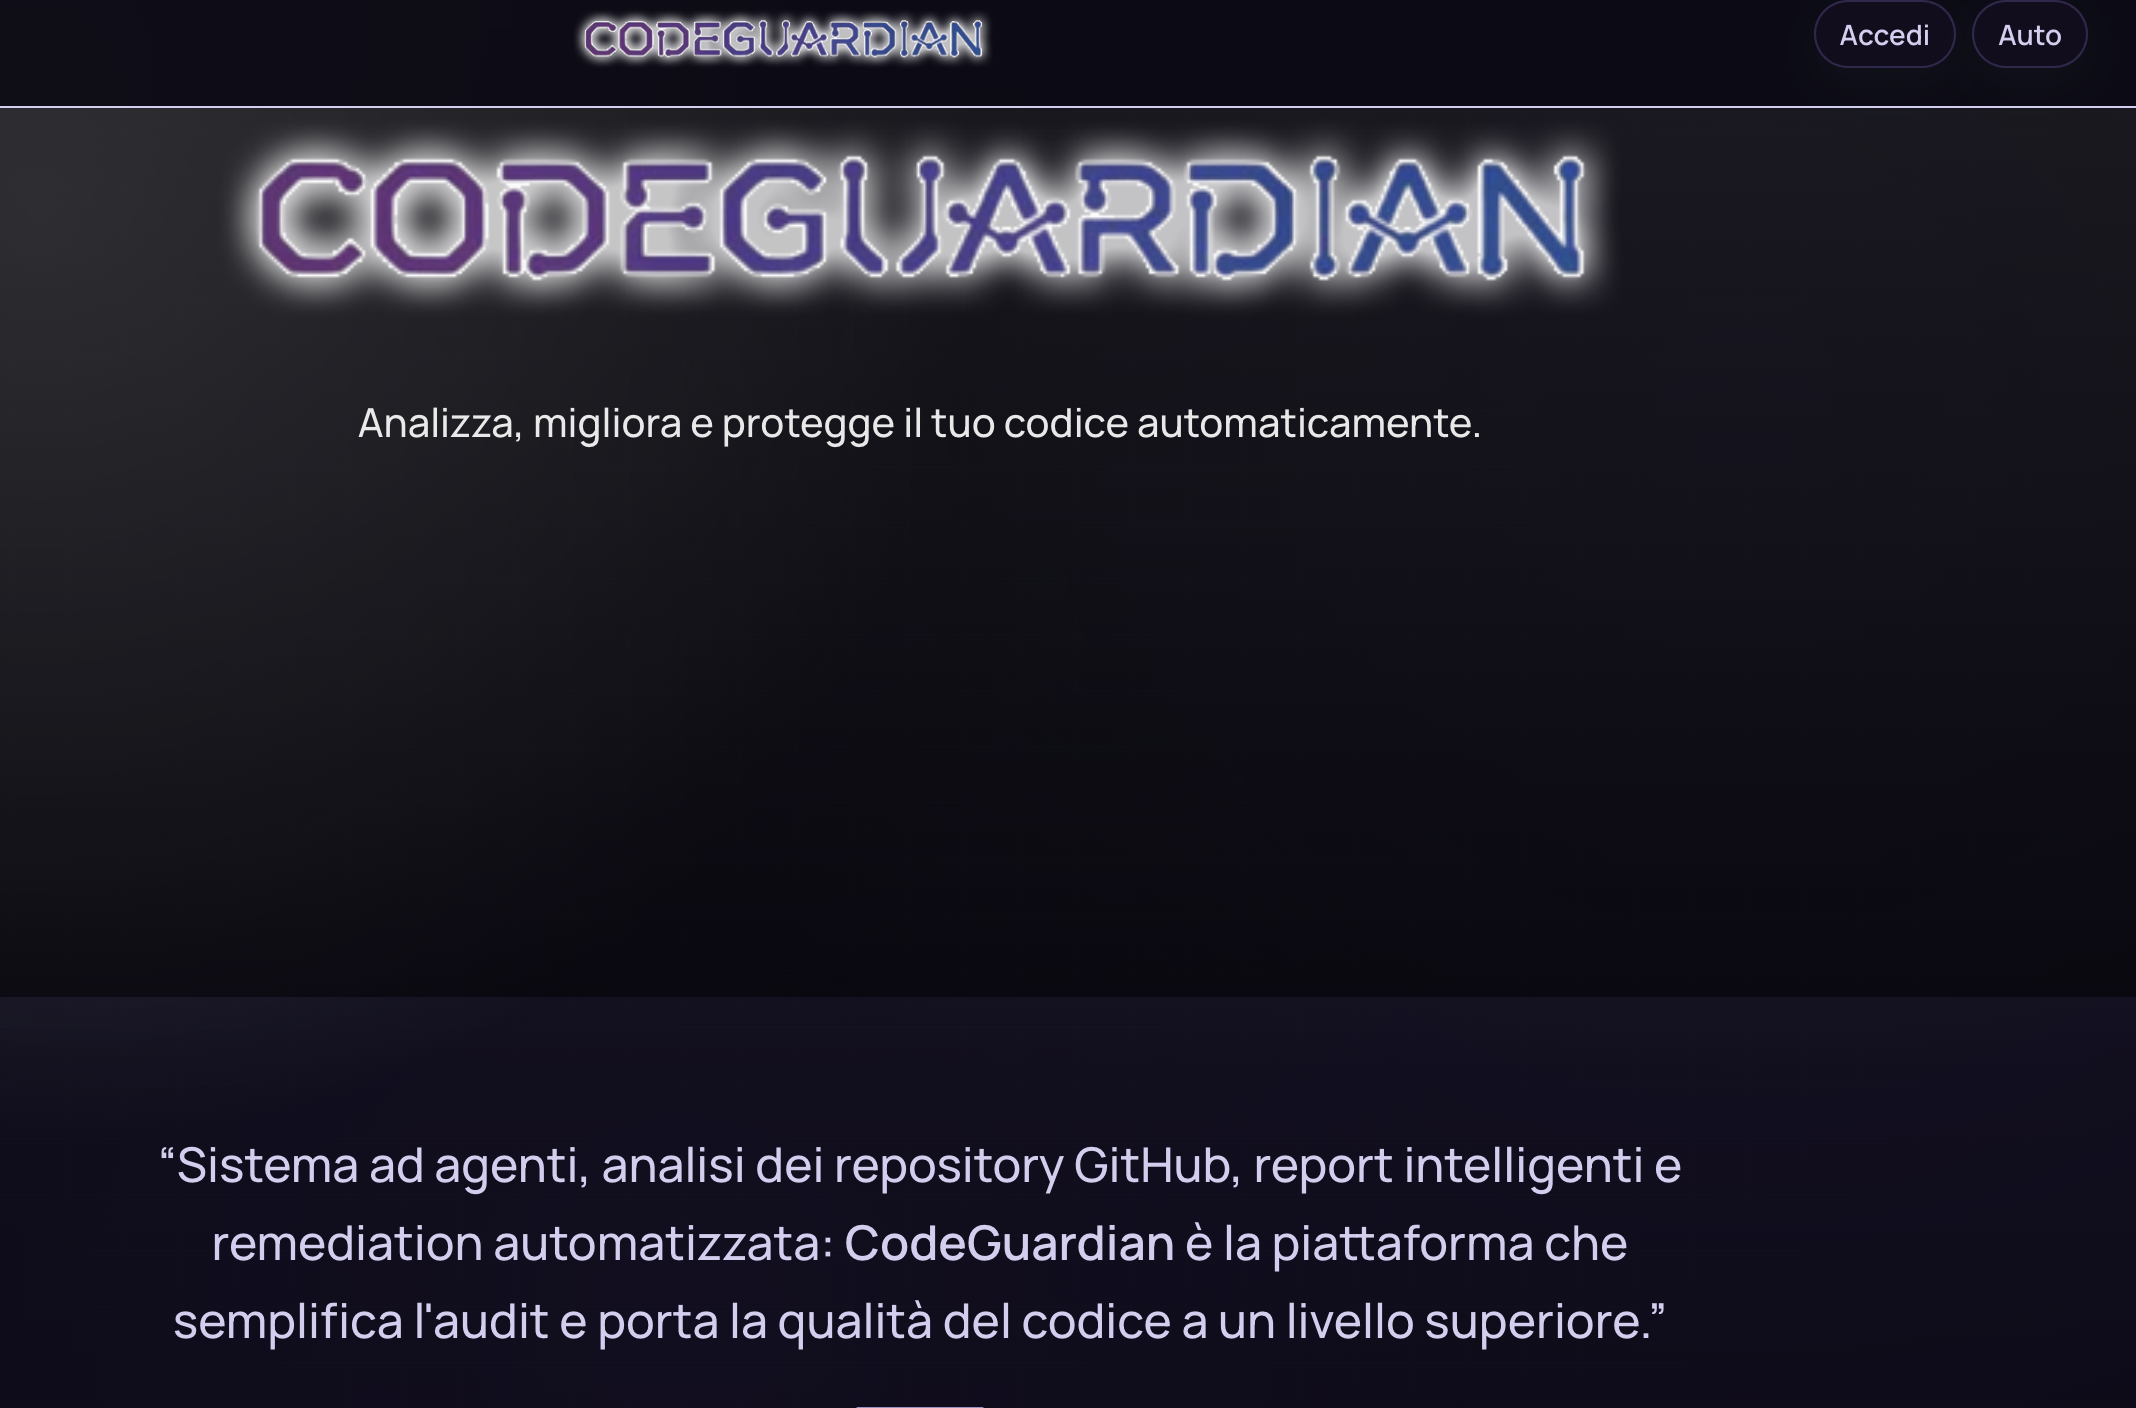
\includegraphics[width=1\textwidth]{../Assets/manuale_utente/homepageCG.png}    
        \caption{Homepage pubblica di CodeGuardian}
    \label{fig:homepage}
\end{figure}
\noindent Per accedere alle funzionalità riservate agli utenti autenticati è necessario cliccare sul pulsante \textbf{Accedi} situato nell'angolo in alto a destra dell'header.
\newpage
\subsection{Login tramite Amazon Cognito}

Cliccando su \textbf{Accedi}, l'utente viene reindirizzato alla pagina di login ospitata da Amazon Cognito\textsuperscript{G}. Qui sarà necessario inserire il nome utente e la password forniti dall'organizzazione.

\begin{figure}[H]
    \centering
        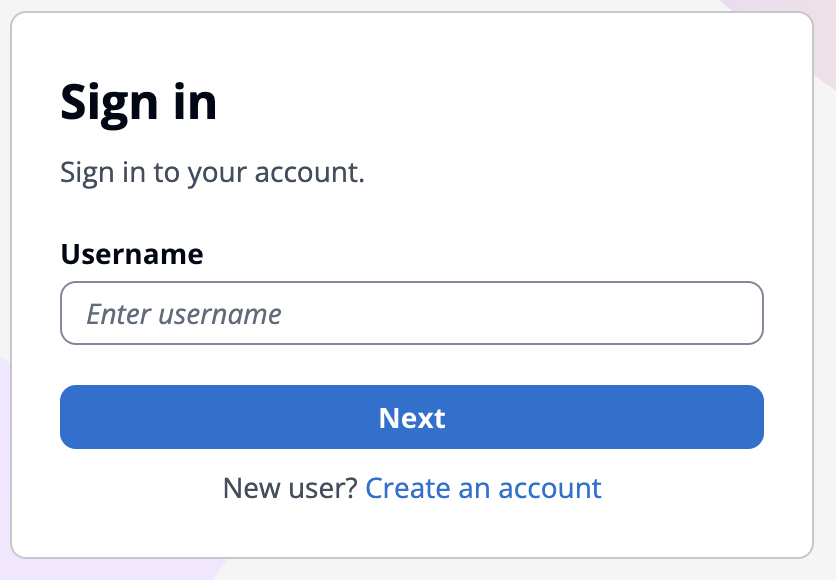
\includegraphics[width=0.5\textwidth]{../Assets/manuale_utente/LoginUserCG.png}    
        \caption{Inserimento username durnate il login}
    \label{fig:LoginUser}
\end{figure}

\begin{figure}[H]
    \centering
        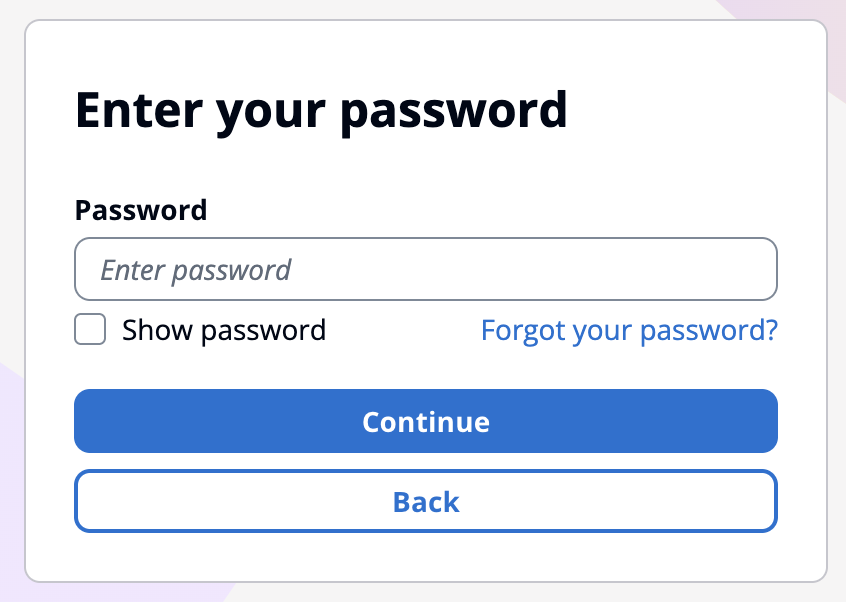
\includegraphics[width=0.5\textwidth]{../Assets/manuale_utente/LoginPswCG.png}    
        \caption{Inserimento password durnate il login}
    \label{fig:LoginPsw}
\end{figure}

\subsection{Callback e registrazione automatica}
\label{sec:callback}

Dopo un login andato a buon fine, il browser viene reindirizzato a una pagina interna di \textit{callback} che mostra il messaggio «Accesso in corso\ldots». In questa fase avvengono, in modo trasparente all'utente:

\begin{enumerate}
    \item il recupero delle informazioni dell'utente autenticato da Cognito;
    \item l'eventuale registrazione dell'utente nel database della piattaforma (solo al primo accesso);
    \item il reindirizzamento alla pagina richiesta prima del login, oppure alla pagina \textbf{Workspace} come destinazione predefinita.
\end{enumerate}

\begin{infobox}
\textbf{Nota:} Se al momento del login l'utente stava tentando di accedere a una pagina protetta (per esempio un link diretto a un report), dopo l'autenticazione verrà ricondotto direttamente a quella pagina.
\end{infobox}

\subsection{Logout}
Per uscire dalla piattaforma, cliccare sul pulsante \textbf{Logout} situato nell'angolo in alto a destra dell'header. Il logout invalida la sessione\textsuperscript{G} corrente su Cognito e riporta l'utente alla homepage pubblica.

\subsection{Gestione degli errori di accesso}
\label{sec:errori-login}

La tabella seguente riassume i principali errori che possono verificarsi durante la fase di autenticazione e le relative soluzioni.

\rowcolors{2}{LightGray}{white}
\begin{longtable}{>{\raggedright\arraybackslash}p{5cm} >{\raggedright\arraybackslash}p{9cm}}
  \rowcolor{AccentColor}
  \textcolor{white}{\textbf{Messaggio / situazione}} &
  \textcolor{white}{\textbf{Causa e risoluzione}} \\
  \endfirsthead

  \rowcolor{AccentColor}
  \textcolor{white}{\textbf{Messaggio / situazione}} &
  \textcolor{white}{\textbf{Causa e risoluzione}} \\
  \endhead

  Credenziali rifiutate da Cognito &
  Username o password non corretti. Verificare le credenziali e riprovare. Dopo ripetuti tentativi falliti l'account potrebbe essere temporaneamente bloccato per motivi di sicurezza. \\
  Reindirizzamento alla homepage con parametro \texttt{?error=registration\_failed} &
  L'autenticazione su Cognito è andata a buon fine, ma la registrazione dell'utente nel database interno è fallita. Per sicurezza l'utente viene rimosso anche da Cognito. Riprovare ad accedere; se il problema persiste, contattare l'amministratore della piattaforma. \\
  Reindirizzamento alla homepage senza errore &
  Cognito ha rifiutato la sessione (ad esempio perché il token è scaduto o perché l'utente ha annullato il login). È sufficiente cliccare nuovamente su \textbf{Accedi}. \\
  La pagina resta bloccata su «Accesso in corso\ldots» &
  Possibile problema di connessione con Cognito o con il backend di CodeGuardian. Ricaricare la pagina; se il problema persiste, controllare la connessione e riprovare più tardi. \\
  Sessione scaduta mentre si utilizza la piattaforma &
  Le sessioni hanno durata limitata. In caso di scadenza, alcune chiamate restituiranno errore e l'utente verrà invitato a effettuare nuovamente il login. \\
\caption{Errori comuni nel flusso di autenticazione}
\label{tab:errori-auth}
\end{longtable}

\newpage
% =====================================================================
\section{Interfaccia utente}
% =====================================================================

\subsection{Struttura generale delle pagine}
Tutte le pagine autenticate di CodeGuardian condividono la stessa struttura:
\begin{itemize}
    \item \textbf{Header superiore}: contiene, da sinistra a destra, i link rapidi a \textbf{Workspace} e \textbf{Inviti}, il logo della piattaforma (link alla homepage), il pulsante \textbf{+ New Workspace}, il pulsante \textbf{Logout} e il selettore del tema;
    \item \textbf{Area centrale}: il contenuto specifico della pagina (lista workspace, dettaglio repository, report, ecc.);
    \item \textbf{Footer inferiore}: contiene il logo e il nome della piattaforma, il riferimento al gruppo Byte-Holders e l'anno di copyright.
\end{itemize}

\begin{figure}[H]
    \centering
        
\includegraphics[width=1\textwidth]{../Assets/manuale_utente/HeaderCG.png}    
        \caption{Header con navigazione, logo centrale e pulsanti a destra}
    \label{fig:Header}
\end{figure}

\subsection{Selezione del tema}
CodeGuardian supporta tre modalità di visualizzazione, selezionabili tramite il pulsante a destra dell'header:
\begin{itemize}
    \item \textbf{Light}: tema chiaro;
    \item \textbf{Dark}: tema scuro;
    \item \textbf{Auto}: il tema segue le impostazioni di sistema del dispositivo.
\end{itemize}

La preferenza selezionata viene memorizzata nel browser e mantenuta fra le sessioni.

\subsection{Navigazione principale}
I due link della barra di navigazione permettono di raggiungere rapidamente le pagine principali della piattaforma:
\begin{itemize}
    \item \textbf{Workspace}: pagina con la lista dei workspace di cui si è membri;
    \item \textbf{Inviti}: pagina con la lista degli inviti pendenti ricevuti da altri utenti.
\end{itemize}

Il logo al centro dell'header funge da link alla homepage pubblica.

\newpage
% =====================================================================
\section{Gestione dei workspace}
% =====================================================================

\subsection{Lista dei workspace}
Dopo l'accesso l'utente visualizza la pagina \textbf{Workspace}, che riporta in forma di schede tutti i workspace\textsuperscript{G} di cui è membro.


\begin{figure}[H]
    \centering
        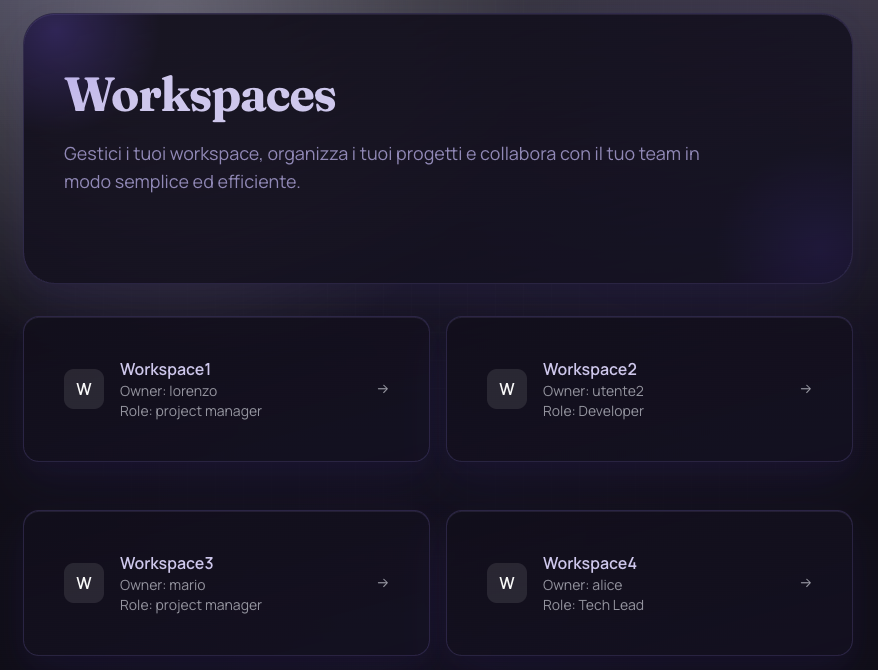
\includegraphics[width=0.8\textwidth]{../Assets/manuale_utente/workspaceList.png}    
        \caption{Pagina lista workspace}
    \label{fig:lista-workspace}
\end{figure}


\noindent Ogni scheda mostra:
\begin{itemize}
    \item un'icona con la prima lettera del nome del workspace;
    \item il nome del workspace;
    \item il nome dell'owner\textsuperscript{G};
    \item il ruolo dell'utente corrente all'interno di quel workspace.
\end{itemize}
Cliccando su una scheda si accede al dettaglio del workspace, dove sono visibili le relative liste di repository e di membri.
Se l'utente non fa ancora parte di alcun workspace, al centro della pagina viene mostrato il messaggio «\textit{No workspaces yet. Create your first one!}».
\newpage
\subsection{Creazione di un nuovo workspace}
Per creare un nuovo workspace:
\begin{enumerate}
    \item cliccare sul pulsante \textbf{+ New Workspace} nell'header;
    \item nella finestra di dialogo che appare, inserire il nome del workspace nel campo \textbf{Workspace Name};
    \item cliccare su \textbf{Create Workspace} per confermare, oppure su \textbf{Cancel} per annullare l'operazione.
\end{enumerate}


\begin{figure}[H]
    \centering
        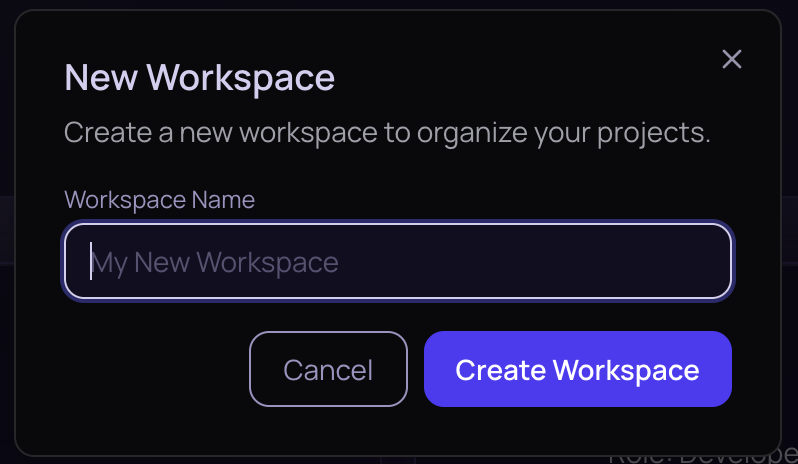
\includegraphics[width=0.8\textwidth]{../Assets/manuale_utente/newWorkspace.png}    
        \caption{Dialog di creazione workspace}
    \label{fig:new-workspace}
\end{figure}
\begin{infobox}
\textbf{Vincoli sul nome.} Il nome del workspace deve avere lunghezza compresa fra 2 e 30 caratteri. In caso di valore non valido, sotto il campo di testo viene mostrato il messaggio di errore corrispondente.
\end{infobox}
\noindent Dopo la conferma, l'utente viene reindirizzato alla pagina dei repository del nuovo workspace. L'utente creatore è automaticamente:
\begin{itemize}
    \item owner\textsuperscript{G} del workspace;
    \item membro del workspace con ruolo predefinito.
\end{itemize}

\subsection{Header del workspace}
All'interno di un workspace, nella parte superiore della pagina viene mostrato un header dedicato che contiene:
\begin{itemize}
    \item l'avatar del workspace (iniziali del nome), cliccabile per tornare alla lista dei repository;
    \item il nome del workspace;
    \item un badge colorato che indica il ruolo dell'utente corrente (Project Manager, Tech Lead o Developer);
    \item il numero totale di membri;
    \item il numero totale di repository;
\end{itemize}

\begin{figure}[H]
    \centering
        
\includegraphics[width=0.8\textwidth]{../Assets/manuale_utente/WorkspaceHeader.png}    
        \caption{Header di un workspace}
    \label{fig:header-workspace}
\end{figure}

\subsection{Eliminazione di un workspace}

\begin{rolebox}{Owner\textsuperscript{G} del workspace}
Solo l'utente che ha creato il workspace può eliminarlo.
\end{rolebox}

Per eliminare un workspace:
\begin{enumerate}
    \item aprire l'header del workspace;
    \item cliccare sul pulsante rosso \textbf{Elimina};
    \item nella finestra di conferma, cliccare su \textbf{Elimina} per confermare o su \textbf{Annulla} per annullare l'operazione.
\end{enumerate}

\begin{warnbox}
\textbf{Attenzione: operazione irreversibile.} L'eliminazione di un workspace rimuove definitivamente tutti i repository ad esso associati, tutti i membri e tutti i report storici. Non è possibile ripristinare un workspace eliminato.
\end{warnbox}

\noindent Al termine dell'eliminazione, l'utente viene reindirizzato alla pagina \textbf{Workspace}.

\subsection{Navigazione fra le sezioni del workspace}
All'interno di un workspace sono disponibili due sezioni principali, accessibili tramite i link in alto a destra nella pagina della lista repository:
\begin{itemize}
    \item \textbf{Repository}: elenco dei repository (è la pagina predefinita);
    \item \textbf{Membri}: elenco dei membri del workspace e pannello di invito.
\end{itemize}

\newpage
% =====================================================================
\section{Gestione dei membri e degli inviti}
% =====================================================================

\subsection{Pagina «Inviti»}
Cliccando sul link \textbf{Inviti} nell'header, l'utente accede alla pagina che elenca tutti gli inviti pendenti ricevuti da altri utenti.

\begin{figure}[H]
\centering
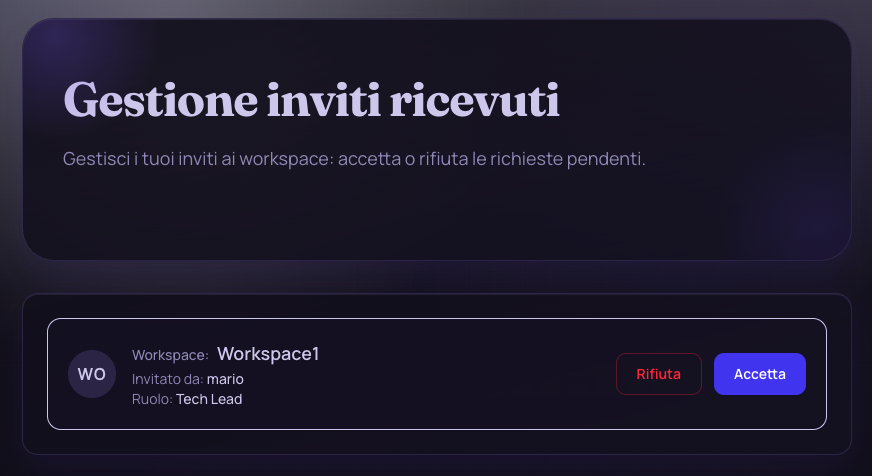
\includegraphics[width=0.8\textwidth]{../Assets/manuale_utente/GestioneInviti.png}    
\caption{Pagina degli inviti ricevuti}
\label{fig:inviti}
\end{figure}

\noindent Ogni invito riporta:
\begin{itemize}
    \item un'icona con le iniziali del workspace;
    \item il nome del workspace;
    \item il nome dell'utente mittente dell'invito;
    \item il ruolo che verrà assegnato all'utente se l'invito viene accettato.
\end{itemize}

\noindent Se non ci sono inviti pendenti, viene mostrato il messaggio «\textit{Nessun invito pendente}».

\subsection{Accettare o rifiutare un invito}
Per ciascun invito sono disponibili due pulsanti:
\begin{itemize}
    \item \textbf{Accetta}: l'utente viene aggiunto al workspace con il ruolo indicato e l'invito scompare dalla lista;
    \item \textbf{Rifiuta}: l'invito viene marcato come rifiutato e scompare dalla lista.
\end{itemize}

\noindent Durante l'elaborazione della scelta, entrambi i pulsanti vengono temporaneamente disabilitati per evitare azioni duplicate.

\begin{infobox}
\textbf{Nota.} Una volta accettato, un invito non può essere annullato. Per uscire da un workspace in cui si è stati aggiunti è necessario chiedere a un amministratore di rimuoverci tramite la pagina dei membri.
\end{infobox}

\newpage
\subsection{Pagina «Membri»}
\label{sec:membri}

La pagina \textbf{Membri} di un workspace è raggiungibile dal link \textbf{Membri} presente nella pagina della lista repository. La pagina è suddivisa in due aree:
\begin{enumerate}
    \item nella parte alta, il form di invito;
    \item nella parte bassa, la lista dei membri correnti del workspace.
\end{enumerate}

\begin{figure}[H]
\centering
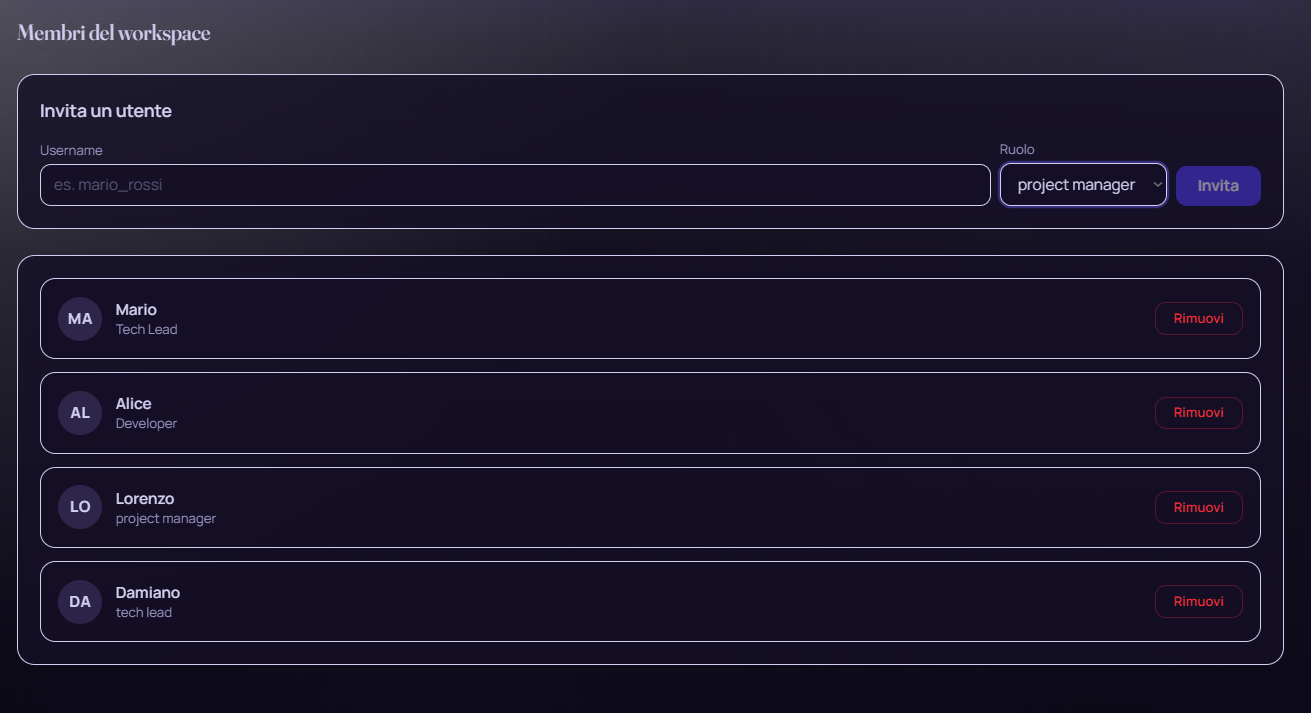
\includegraphics[width=0.8\textwidth]{../Assets/manuale_utente/GestioneMembri.png}    
\caption{Pagina gestione membri di un workspace}
\label{fig:membri}
\end{figure}

\subsection{Invitare un utente al workspace}
\label{sec:invita-utente}

\begin{rolebox}{Project Manager\textsuperscript{G} o owner\textsuperscript{G} del workspace}
L'invio di inviti è tipicamente riservato a chi gestisce il workspace.
\end{rolebox}

\noindent Per invitare un utente:
\begin{enumerate}
    \item accedere alla pagina \textbf{Membri} del workspace;
    \item nel campo \textbf{Username} inserire l'username esatto dell'utente da invitare (lo stesso che l'utente usa per accedere a CodeGuardian);
    \item nel menu a tendina \textbf{Ruolo} selezionare uno fra: \textit{project manager}, \textit{tech lead} e \textit{developer};
    \item cliccare sul pulsante \textbf{Invita}.
\end{enumerate}

\noindent A conferma dell'operazione viene mostrato il messaggio «\textit{Invito inviato con successo}». L'utente destinatario troverà l'invito nella propria pagina \textbf{Inviti}.

\newpage
\subsection{Errori comuni nell'invio degli inviti}

\rowcolors{2}{LightGray}{white}
\begin{longtable}{>{\raggedright\arraybackslash}p{5cm} >{\raggedright\arraybackslash}p{9cm}}
  \rowcolor{AccentColor}
  \textcolor{white}{\textbf{Errore}} &
  \textcolor{white}{\textbf{Causa e risoluzione}} \\
  \endfirsthead

  \rowcolor{AccentColor}
  \textcolor{white}{\textbf{Errore}} &
  \textcolor{white}{\textbf{Causa e risoluzione}} \\
  \endhead

  Il pulsante \textbf{Invita} è disabilitato &
  Il campo \textbf{Username} è vuoto o contiene solo spazi. Inserire un valore valido. \\
  Messaggio di errore rosso sotto il form &
  L'username inserito non corrisponde a nessun utente registrato, oppure l'utente è già membro del workspace, oppure esiste già un invito pendente per quello stesso utente. Verificare l'username e ricontrollare la lista membri/inviti. \\
  L'invito non compare all'utente destinatario &
  L'invito viene caricato al momento di aprire la pagina \textbf{Inviti}. Chiedere all'utente di aggiornare la pagina. \\
\caption{Errori nell'invio degli inviti}
\label{tab:errori-inviti}
\end{longtable}

\subsection{Rimuovere un membro dal workspace}

\begin{rolebox}{Project Manager\textsuperscript{G} o owner\textsuperscript{G} del workspace}
Generalmente riservato a chi gestisce il workspace.
\end{rolebox}

\noindent Nella lista dei membri, a fianco di ciascun utente, è presente il pulsante rosso \textbf{Rimuovi}. Cliccandolo, l'utente viene rimosso dal workspace; il pulsante è temporaneamente disabilitato durante l'operazione.

\begin{warnbox}
\textbf{Attenzione.} La rimozione di un membro è immediata e non prevede conferma esplicita. L'utente rimosso perde l'accesso al workspace e ai relativi repository e report. Può essere reinvitato successivamente seguendo la procedura descritta nella sezione~\ref{sec:invita-utente}.
\end{warnbox}

\subsection{Stati degli inviti}
Ogni invito attraversa, dal punto di vista del sistema, tre stati possibili:
\begin{itemize}
    \item \textbf{PENDING}: invito inviato e in attesa di risposta; visibile nella pagina \textbf{Inviti} del destinatario;
    \item \textbf{ACCEPTED}: invito accettato; non più visibile nella lista, l'utente è aggiunto al workspace;
    \item \textbf{REJECTED}: invito rifiutato; non più visibile nella lista, l'utente non è aggiunto al workspace.
\end{itemize}

\newpage
% =====================================================================
\section{Gestione dei repository}
% =====================================================================

\subsection{Pagina lista repository}
All'interno di un workspace, la pagina dei \textbf{Repository} mostra tutti i repository\textsuperscript{G} GitHub che sono stati aggiunti al workspace. La pagina include:
\begin{itemize}
    \item un titolo \textbf{Lista repository};
    \item un link rapido alla pagina \textbf{Membri};
    \item un form di aggiunta di un nuovo repository;
    \item una barra di ricerca per filtrare i repository per nome;
    \item l'elenco dei repository sotto forma di schede.
\end{itemize}

\begin{figure}[H]
\centering
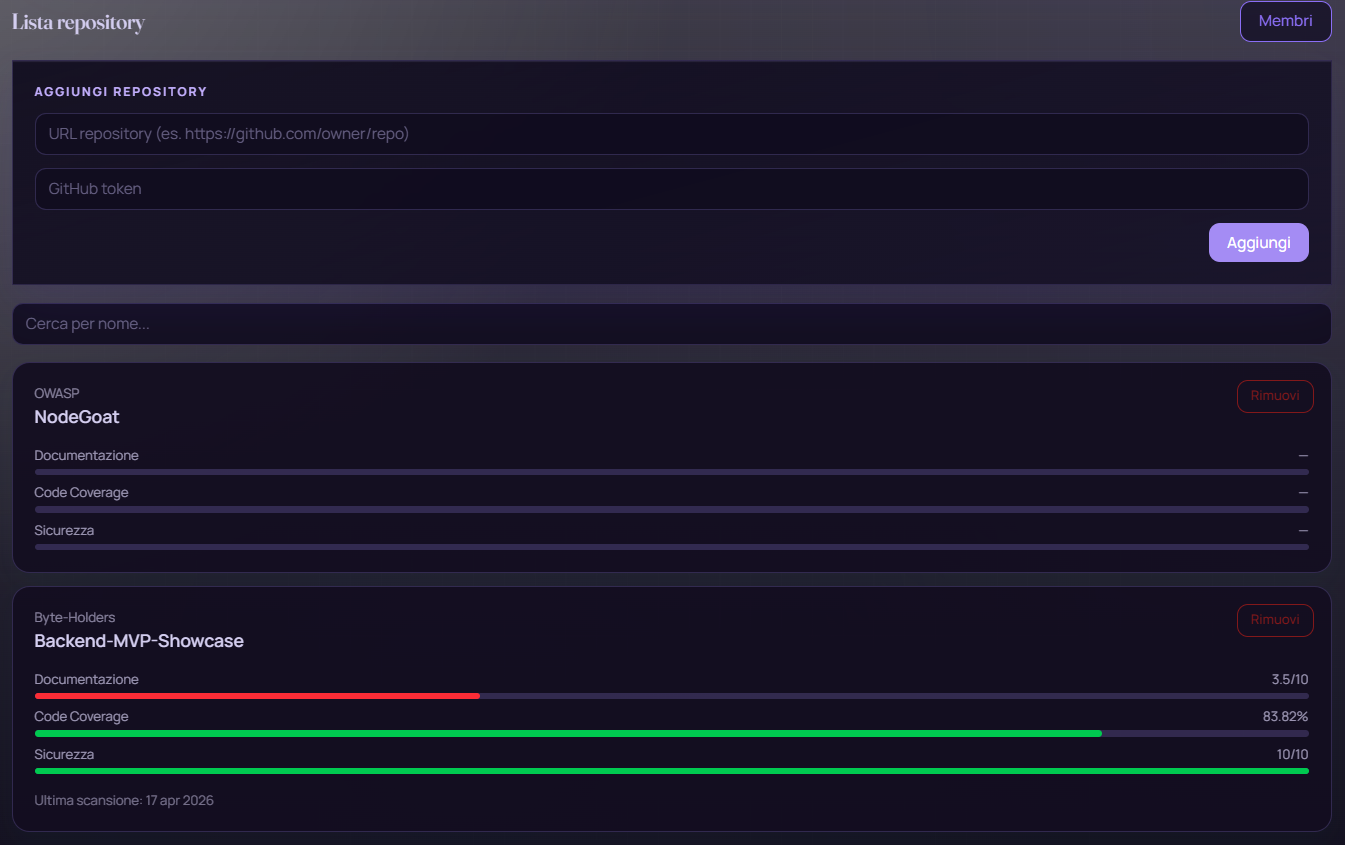
\includegraphics[width=0.9\textwidth]{../Assets/manuale_utente/ListaRepo.png}    
\caption{Lista repository di un workspace}
\label{fig:lista-repository}
\end{figure}

Ogni scheda riporta, se disponibili:
\begin{itemize}
    \item il nome del proprietario GitHub del repository;
    \item il nome del repository;
    \item il punteggio di \textbf{Documentazione} (scala 0--10);
    \item il valore di \textbf{Code Coverage} (scala 0--100\%);
    \item il punteggio di \textbf{Sicurezza} (scala 0--10);
    \item la data dell'ultima scansione;
    \item un pulsante \textbf{Rimuovi} per eliminare il repository dal workspace.
\end{itemize}

Se non ci sono repository viene mostrato il messaggio «\textit{Nessun repository aggiunto}».


\begin{warnbox}
\textbf{Attenzione.} Nel caso non ci fosse un report disponibile del branch di develop non saranno visibili i punteggi di Documentazione, Code Coverage e Sicurezza nella lista dei repository (Come si può vedere dall'immagine~\ref{fig:lista-repository}).
\end{warnbox}

\subsection{Ricerca di un repository}
La barra di ricerca nella parte alta della pagina permette di filtrare i repository per nome. Il filtraggio avviene in tempo reale mentre si digita: sono mostrati solo i repository il cui nome contiene la stringa inserita. Per azzerare il filtro è sufficiente svuotare il campo di testo.

\subsection{Aggiungere un repository}

\begin{rolebox}{Project Manager\textsuperscript{G} o Tech Lead\textsuperscript{G}}
Generalmente il creatore stesso della repository su GitHub\textsuperscript{G}.
\end{rolebox}

\noindent Per aggiungere un repository al workspace:
\begin{enumerate}
    \item nella sezione \textbf{Aggiungi repository}, inserire l'URL del repository GitHub\textsuperscript{G} nel campo \textbf{URL repository} (esempio: \texttt{https://github.com/owner/nome-repo});
    \item se il repository è privato, inserire un Personal Access Token\textsuperscript{G} GitHub nel campo \textbf{GitHub token} (si veda la sezione~\ref{sec:token});
    \item cliccare su \textbf{Aggiungi}.
\end{enumerate}

\begin{figure}[H]
\centering
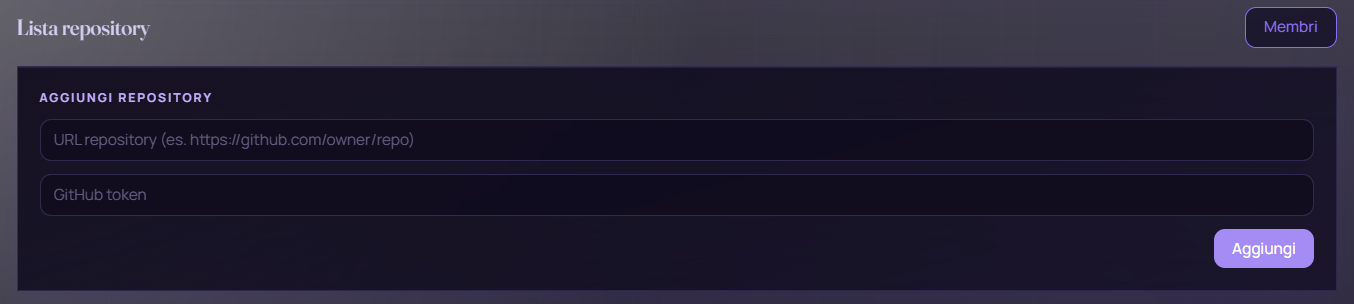
\includegraphics[width=1\textwidth]{../Assets/manuale_utente/AggiuntaRepo.png}    
\caption{Form di aggiunta di un nuovo repository}
\label{fig:add-repository}
\end{figure}

\noindent Durante l'aggiunta il pulsante si trasforma in «\textit{Aggiunta\ldots}» e resta disabilitato. In caso di successo, il nuovo repository appare immediatamente nella lista e i campi del form vengono svuotati.

\newpage
\subsection{Errori comuni nell'aggiunta di un repository}

\rowcolors{2}{LightGray}{white}
\begin{longtable}{>{\raggedright\arraybackslash}p{5cm} >{\raggedright\arraybackslash}p{9cm}}
  \rowcolor{AccentColor}
  \textcolor{white}{\textbf{Errore}} &
  \textcolor{white}{\textbf{Causa e risoluzione}} \\
  \endfirsthead

  \rowcolor{AccentColor}
  \textcolor{white}{\textbf{Errore}} &
  \textcolor{white}{\textbf{Causa e risoluzione}} \\
  \endhead

  «URL non valido» &
  L'URL inserito non ha il formato corretto. Verificare che inizi con \texttt{https://github.com/} e sia seguito da \texttt{owner/repository}. \\
  «Repository non trovato» &
  Il repository non esiste su GitHub oppure è privato e il token non è stato fornito. Controllare l'URL o fornire un Personal Access Token valido. \\
  «Token non autorizzato» &
  Il token fornito non ha i permessi di lettura sul repository indicato. Generare un nuovo token con scope \texttt{repo}. \\
  «Repository già presente» &
  Il repository è già stato aggiunto a questo workspace. Utilizzare la barra di ricerca per individuarlo nella lista esistente. \\
  Il pulsante \textbf{Aggiungi} resta su «\textit{Aggiunta\ldots}» &
  Problema temporaneo di connessione. Attendere qualche secondo; se il problema persiste, ricaricare la pagina. \\
\caption{Errori nell'aggiunta di un repository}
\label{tab:errori-add-repo}
\end{longtable}

\subsection{Aggiornare il token di un repository}
\label{sec:token}

Il Personal Access Token\textsuperscript{G} (PAT) è un token di autenticazione generato da GitHub che permette a CodeGuardian di accedere al codice di repository privati. I formati accettati sono:
\begin{itemize}
    \item \textbf{Classic token}: inizia con \texttt{ghp\_} seguito da 36 caratteri alfanumerici;
    \item \textbf{Fine-grained token}: inizia con \texttt{github\_pat\_} seguito da 82 caratteri fra lettere, numeri e underscore.
\end{itemize}

\begin{rolebox}{Project Manager\textsuperscript{G} o Tech Lead\textsuperscript{G}}
Rimane fondamentale avere a disposizione un PAT di un account GitHub con i corretti permessi in modo da eseguire lo scan senza interruzioni.
\end{rolebox}

\noindent Per aggiornare o inserire un nuovo token su un repository già presente:
\begin{enumerate}
    \item aprire la pagina di dettaglio del repository (cliccandoci sopra dalla lista);
    \item nell'header, accanto al nome del repository, cliccare sull'icona a forma di chiave;
    \item nel campo che appare, incollare il token;
    \item cliccare su \textbf{Salva}.
\end{enumerate}

\begin{figure}[H]
\centering
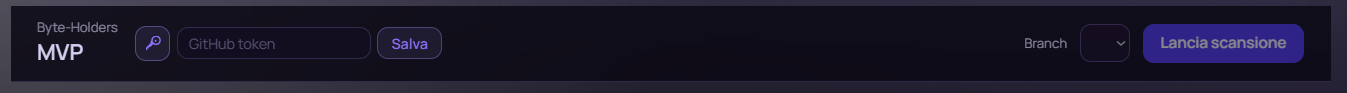
\includegraphics[width=0.95\textwidth]{../Assets/manuale_utente/TokenInline.png}    
\caption{Form di aggiornamento del GitHub token}
\label{fig:update-token}
\end{figure}

\begin{warnbox}
\textbf{Messaggio «Token non valido».} Se il token non rispetta uno dei due formati attesi, il client mostra l'errore «\textit{Token non valido}» prima di inviare la richiesta al server. Verificare il formato e riprovare.
\end{warnbox}

\noindent In caso di errore lato server, il messaggio di errore restituito dal backend viene mostrato sotto il campo di testo (per esempio se il token non ha i permessi necessari sul repository).

\subsection{Rimuovere un repository}

\begin{rolebox}{Project Manager\textsuperscript{G} o Tech Lead\textsuperscript{G}}
Generalmente la stessa persona che ha aggiunto la repository nel Workspace.
\end{rolebox}

\noindent Per rimuovere un repository dal workspace è sufficiente cliccare sul pulsante \textbf{Rimuovi} presente nell'angolo in alto a destra della scheda del repository, sia dalla lista sia dalla pagina di dettaglio.

\begin{warnbox}
\textbf{Attenzione: operazione non reversibile.} L'eliminazione rimuove dal workspace il repository e tutti i report storici ad esso associati. Per reinserire il repository sarà necessario ripetere la procedura di aggiunta dalla sezione apposita.
\end{warnbox}

\noindent Durante la rimozione il pulsante mostra «\textit{Rimozione\ldots}» e resta disabilitato. Al termine il repository scompare dalla lista.

\newpage
% =====================================================================
\section{Esecuzione di una scansione}
% =====================================================================

\subsection{Pagina di dettaglio del repository}
Cliccando su un repository nella lista si accede alla pagina di dettaglio (\textbf{Report}), che contiene:
\begin{itemize}
    \item l'header con il nome del proprietario GitHub, il nome del repository e il pulsante per aggiornare il token;
    \item il selettore di \textbf{Branch};
    \item il pulsante per avviare o fermare la scansione\textsuperscript{G};
    \item il corpo del report generato dall'ultima scansione (se disponibile).
\end{itemize}

\begin{figure}[H]
\centering
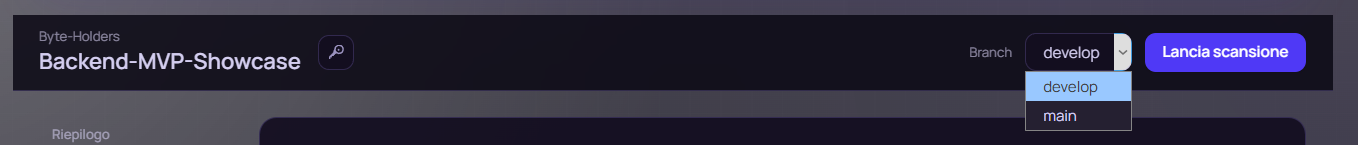
\includegraphics[width=0.95\textwidth]{../Assets/manuale_utente/HeaderDettaglioRepo.png}    
\caption{Header della pagina di dettaglio repository}
\label{fig:repo-header}
\end{figure}

\subsection{Selezione del branch}
Il menu a tendina \textbf{Branch} permette di scegliere il branch\textsuperscript{G} del repository su cui eseguire la scansione (o di cui visualizzare il report).
\begin{itemize}
    \item Se il repository contiene un branch chiamato \texttt{develop}, viene selezionato automaticamente.
    \item Altrimenti viene selezionato il primo branch disponibile.
    \item L'utente può comunque cambiare la selezione in qualsiasi momento tramite il menu.
\end{itemize}

\begin{infobox}
\textbf{Nota.} Se l'utente cambia branch mentre una scansione è in corso, la scansione continuerà sul branch originariamente scelto. Per scansionare un altro branch è necessario aspettare (o fermare) la scansione corrente e avviarne una nuova.
\end{infobox}

\subsection{Avvio di una scansione}
Per avviare una scansione:
\begin{enumerate}
    \item selezionare il branch desiderato dal menu \textbf{Branch};
    \item cliccare sul pulsante \textbf{Lancia scansione} in alto a destra.
\end{enumerate}

Durante l'avvio il pulsante mostra «\textit{Avvio\ldots}» e resta disabilitato. Quando la scansione è stata correttamente avviata, il pulsante si trasforma nel pulsante rosso \textbf{Ferma scansione}.

\begin{figure}[H]
\centering

\includegraphics[width=0.95\textwidth]{../Assets/manuale_utente/FermaScansione.png}    
\caption{Stato «scansione in corso»}
\label{fig:scan-running}
\end{figure}

\begin{infobox}
\textbf{Durata tipica.} Una scansione richiede tipicamente fra i due e tre minuti. Durante questo intervallo la pagina rimane utilizzabile ed è possibile navigare fra i report dei branch già scansionati.
\end{infobox}

\subsection{Interruzione di una scansione}
Cliccando su \textbf{Ferma scansione} durante un'esecuzione, la scansione viene interrotta e il pulsante mostra temporaneamente «\textit{Arresto\ldots}» prima di tornare a \textbf{Lancia scansione}.

\begin{warnbox}
\textbf{Attenzione.} Interrompere una scansione non produce alcun nuovo report: lo stato del report visualizzato resterà quello dell'ultima scansione completata con successo.
\end{warnbox}

\subsection{Stati della scansione}
Durante la sua esecuzione una scansione transita attraverso diversi stati. I tre stati terminali che determinano la fine della scansione sono:
\begin{itemize}
    \item \textbf{completed}: la scansione è terminata con successo; il nuovo report è disponibile;
    \item \textbf{stopped}: la scansione è stata interrotta dall'utente prima del termine;
    \item \textbf{error}: la scansione si è interrotta a causa di un errore; il report non è aggiornato.
\end{itemize}

\noindent Quando la scansione raggiunge uno di questi tre stati, il pulsante torna a mostrare \textbf{Lancia scansione}.

\subsection{Fallback automatico}
Per garantire la consistenza dell'interfaccia, qualora l'aggiornamento di stato dovesse tardare, CodeGuardian implementa un meccanismo di fallback: trascorsi 90 secondi dall'avvio della scansione, il client inizia a richiedere periodicamente (ogni 8 secondi) il report del branch corrente. Non appena il report aggiornato è disponibile, lo stato della scansione viene considerato completato.

\subsection{Errori comuni durante la scansione}

\rowcolors{2}{LightGray}{white}
\begin{longtable}{>{\raggedright\arraybackslash}p{5cm} >{\raggedright\arraybackslash}p{9cm}}
  \rowcolor{AccentColor}
  \textcolor{white}{\textbf{Situazione}} &
  \textcolor{white}{\textbf{Causa e risoluzione}} \\
  \endfirsthead

  \rowcolor{AccentColor}
  \textcolor{white}{\textbf{Situazione}} &
  \textcolor{white}{\textbf{Causa e risoluzione}} \\
  \endhead

  Il pulsante \textbf{Lancia scansione} è disabilitato &
  Non è stato selezionato alcun branch, oppure la scansione è già in fase di avvio. Selezionare un branch valido e riprovare. \\
  Errore rosso sotto il pulsante dopo il click su \textbf{Lancia scansione} &
  Il backend ha rifiutato l'avvio (ad esempio: repository non raggiungibile, token invalido, quote esaurite). Leggere il messaggio e adeguarsi: verificare il token, ricaricare la pagina, riprovare più tardi. \\
  Errore rosso dopo il click su \textbf{Ferma scansione} &
  Problema transiente di comunicazione con il backend. Attendere qualche secondo e riprovare. \\
  La scansione resta in «\textit{Ferma scansione}» per molti minuti &
  Dopo 90 secondi il fallback tenta di recuperare il report ogni 8 secondi. Se dopo diversi minuti lo stato non cambia, il backend potrebbe essere bloccato: ricaricare la pagina e riprovare. \\
  Dopo una scansione completata il report non si aggiorna &
  Ricaricare la pagina (F5). Il frontend invalida automaticamente la cache del report al termine della scansione, ma un errore di rete al momento della notifica può impedire il refresh. \\
  «Nessun report disponibile per questo branch» &
  Per il branch selezionato non è mai stata eseguita una scansione completata con successo. Avviarne una tramite \textbf{Lancia scansione}. \\
\caption{Errori nella fase di scansione}
\label{tab:errori-scan}
\end{longtable}

\newpage
% =====================================================================
\section{Visualizzazione del report}
% =====================================================================

\subsection{Struttura generale del report}
Dopo una scansione completata con successo, la pagina di dettaglio del repository mostra il report\textsuperscript{G} generato dagli agenti. La pagina è divisa in due colonne:
\begin{itemize}
    \item una sidebar a sinistra con i link ancora alle sezioni del report;
    \item l'area di contenuto a destra con le varie sezioni in sequenza.
\end{itemize}

Le sezioni sono:
\begin{enumerate}
    \item \textbf{Riepilogo} (mostrata solo se disponibile);
    \item \textbf{Tecnologie};
    \item \textbf{Test};
    \item \textbf{Sicurezza};
    \item \textbf{Documentazione}.
\end{enumerate}

\noindent Cliccando un link della sidebar, la pagina scorre automaticamente fino alla sezione corrispondente.

\subsection{Sezione «Riepilogo»}
La sezione \textbf{Riepilogo}, se presente, contiene:
\begin{itemize}
    \item il \textbf{Voto globale} (scala 0--10) visualizzato all'interno di un indicatore circolare colorato:
    \begin{itemize}
        \item verde/turchese per voti $\geq 7$;
        \item arancio per voti $\geq 5$;
        \item rosso per voti $< 5$;
    \end{itemize}
    \item una descrizione testuale sintetica (supporta formattazione Markdown);
    \item i metadati della scansione: \textbf{Inizio scansione}, \textbf{Fine scansione} e \textbf{Durata} totale.
\end{itemize}

\begin{figure}[H]
\centering
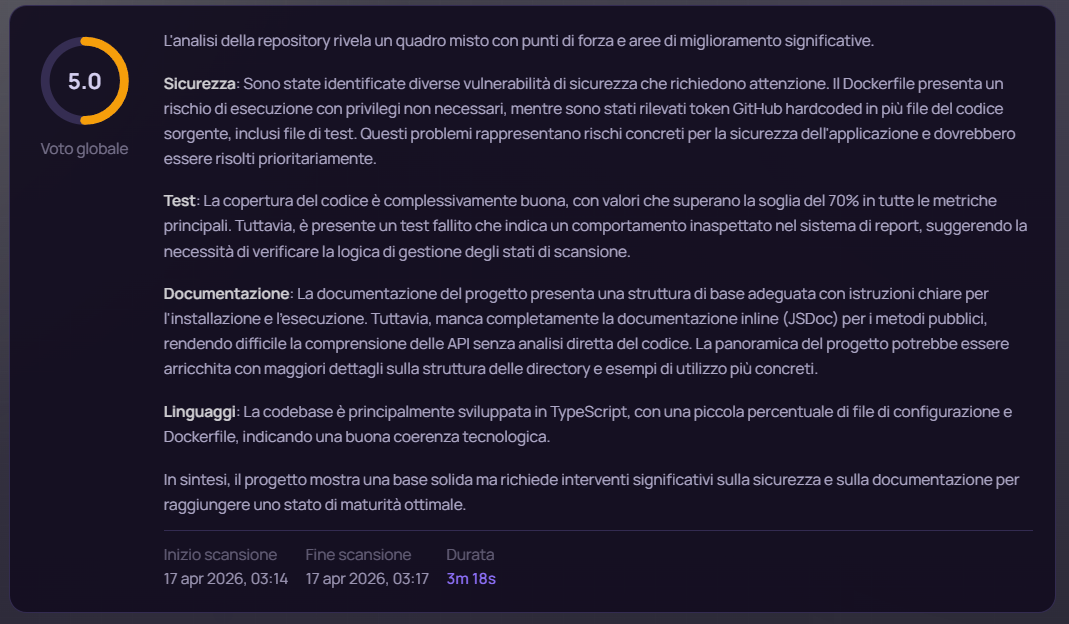
\includegraphics[width=0.7\textwidth]{../Assets/manuale_utente/SezioneRiepilogo.png}    
\caption{Sezione Riepilogo}
\label{fig:report-summary}
\end{figure}

\subsection{Sezione «Tecnologie»}
La sezione fornisce una panoramica dello stack tecnologico rilevato nel repository:
\begin{itemize}
    \item \textbf{Linguaggi}: grafico a torta con la distribuzione percentuale dei linguaggi di programmazione che pesano almeno l'1\%;
    \item linguaggi minori (inferiori all'1\%) mostrati come piccoli chip separati con etichetta «$<1\%$»;
    \item \textbf{Framework}: lista dei framework rilevati con relative versioni;
    \item \textbf{Librerie}: tabella scrollabile con nome e versione delle librerie identificate;
    \item \textbf{Tutte le dipendenze rilevate}: tabella complessiva di tutte le dipendenze del progetto.
\end{itemize}

\begin{figure}[H]
\centering
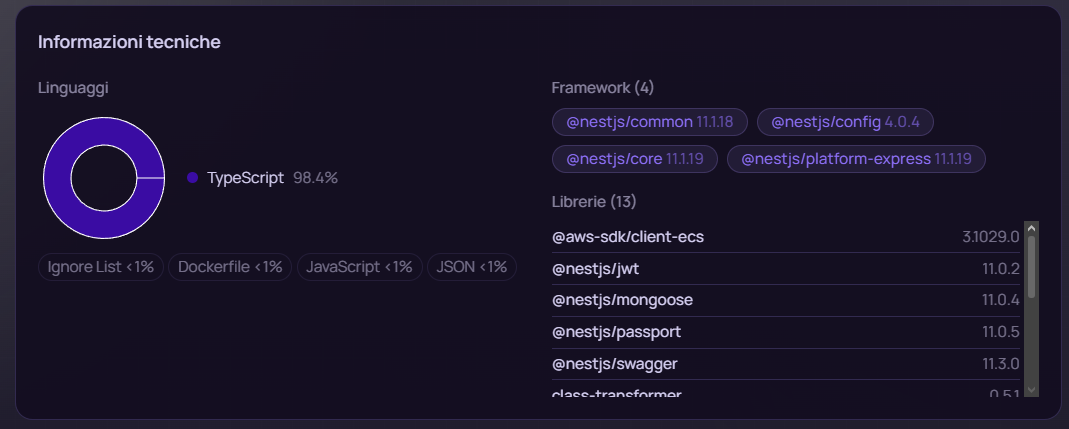
\includegraphics[width=0.85\textwidth]{../Assets/manuale_utente/SezioneTecnologie.png}  
\caption{Sezione Tecnologie}
\label{fig:report-tech}
\end{figure}

Se una categoria non contiene alcun elemento rilevato, viene mostrato il messaggio «Nessuno rilevato» o «Nessuna rilevata».

\subsection{Sezione «Test»}
La sezione fornisce una panoramica della suite di test del progetto:
\begin{itemize}
    \item il totale di \textbf{test eseguiti};
    \item il numero di \textbf{test falliti} (se $> 0$) evidenziato in rosso;
    \item la \textbf{coverage media} e i valori di coverage per le quattro metriche standard: \textbf{Statements}, \textbf{Branches}, \textbf{Functions}, \textbf{Lines};
    \item un grafico a barre con la coverage per ciascuna metrica;
    \item l'elenco dei test falliti, con nome, percorso del file e messaggio riassuntivo.
\end{itemize}

\begin{figure}[H]
\centering
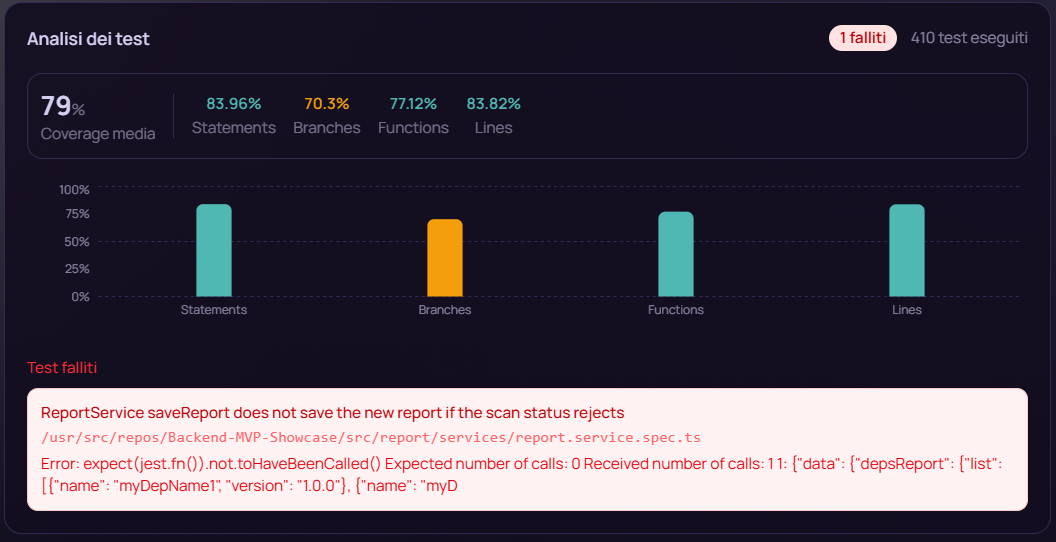
\includegraphics[width=0.8\textwidth]{../Assets/manuale_utente/SezioneCoverage.png}  
\caption{Sezione Test}
\label{fig:report-test}
\end{figure}

\noindent I valori di coverage sono colorati in funzione della soglia:
\begin{itemize}
    \item verde/turchese per valori $\geq 75\%$;
    \item arancio per valori $\geq 50\%$;
    \item rosso per valori $< 50\%$.
\end{itemize}

Se la scansione non rileva alcun test, viene mostrato il messaggio «Nessun test rilevato nel progetto».

\subsection{Sezione «Sicurezza»}
La sezione \textbf{Sicurezza} è la più articolata del report e include:
\begin{enumerate}
    \item un \textbf{voto complessivo di sicurezza del codice}, in scala da 0 a 10, in cui 10 indica una situazione priva di vulnerabilità rilevate;
    \item una panoramica numerica con quattro contatori:
    \begin{itemize}
        \item \textit{Vulnerabilità codice} (totale);
        \item \textit{Critiche (codice)};
        \item \textit{Dipendenze vulnerabili} (totale);
        \item \textit{Critiche (dipendenze)};
    \end{itemize}
    \item due grafici a barre con la distribuzione per severità (Critical / High / Medium / Low) delle vulnerabilità del codice e delle dipendenze;
    \item un'analisi testuale generata dall'agente;
    \item la lista delle \textbf{vulnerabilità nel codice};
    \item la tabella delle \textbf{dipendenze vulnerabili}.
\end{enumerate}

\begin{figure}[H]
\centering
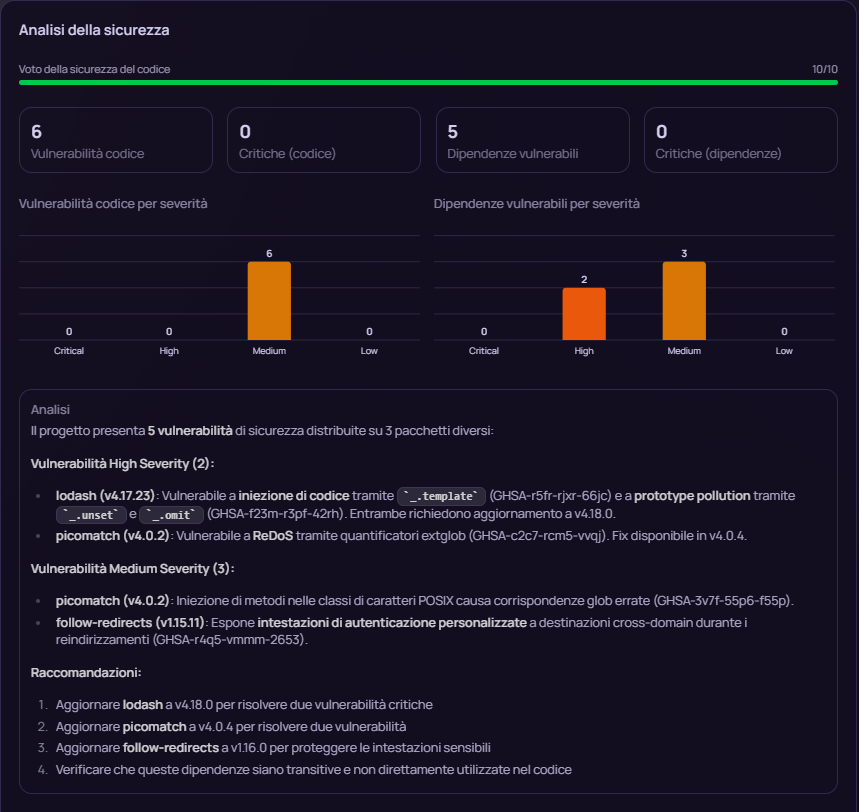
\includegraphics[width=0.6\textwidth]{../Assets/manuale_utente/SezioneSicurezza.png}  
\caption{Sezione Sicurezza}
\label{fig:report-security}
\end{figure}

\subsubsection{Vulnerabilità nel codice}
Ogni vulnerabilità è mostrata come elemento espandibile. Cliccando sull'elemento, vengono rivelati:
\begin{itemize}
    \item il livello di severità (Critical / High / Medium / Low) con colorazione dedicata;
    \item la descrizione del problema;
    \item il percorso del file interessato;
    \item il rimedio suggerito dall'agente (supporta Markdown);
    \item il riferimento CWE\textsuperscript{G} (se disponibile);
    \item uno o più riferimenti alla categoria OWASP\textsuperscript{G} di appartenenza (se disponibili).
\end{itemize}

Una secondo click richiude l'elemento.

\subsubsection{Dipendenze vulnerabili}
Le dipendenze vulnerabili sono raggruppate per pacchetto e versione. Espandendo la sezione \textbf{Dipendenze vulnerabili} viene mostrata una tabella con tre colonne:
\begin{itemize}
    \item \textbf{Pacchetto}: nome e versione del pacchetto;
    \item \textbf{Criticità}: elenco delle vulnerabilità note, ciascuna con un badge di severità e il relativo CVE\textsuperscript{G};
    \item \textbf{Fix}: versione corretta del pacchetto (se disponibile).
\end{itemize}

\noindent Se non sono state rilevate né vulnerabilità nel codice né dipendenze vulnerabili, viene mostrato il messaggio «Nessuna vulnerabilità rilevata».

\subsection{Sezione «Documentazione»}
La sezione \textbf{Documentazione} fornisce un voto (scala 0--10) relativo alla qualità della documentazione del repository, suddiviso in due sotto-analisi:
\begin{itemize}
    \item \textbf{README}: valutazione della completezza e chiarezza del file README del repository;
    \item \textbf{Commenti nel codice}: valutazione della quantità e qualità dei commenti inline nel codice.
\end{itemize}

\noindent Entrambe le sottosezioni presentano un commento testuale generato dall'agente, che può contenere tabelle, liste ed esempi formattati in Markdown.

\begin{figure}[H]
\centering
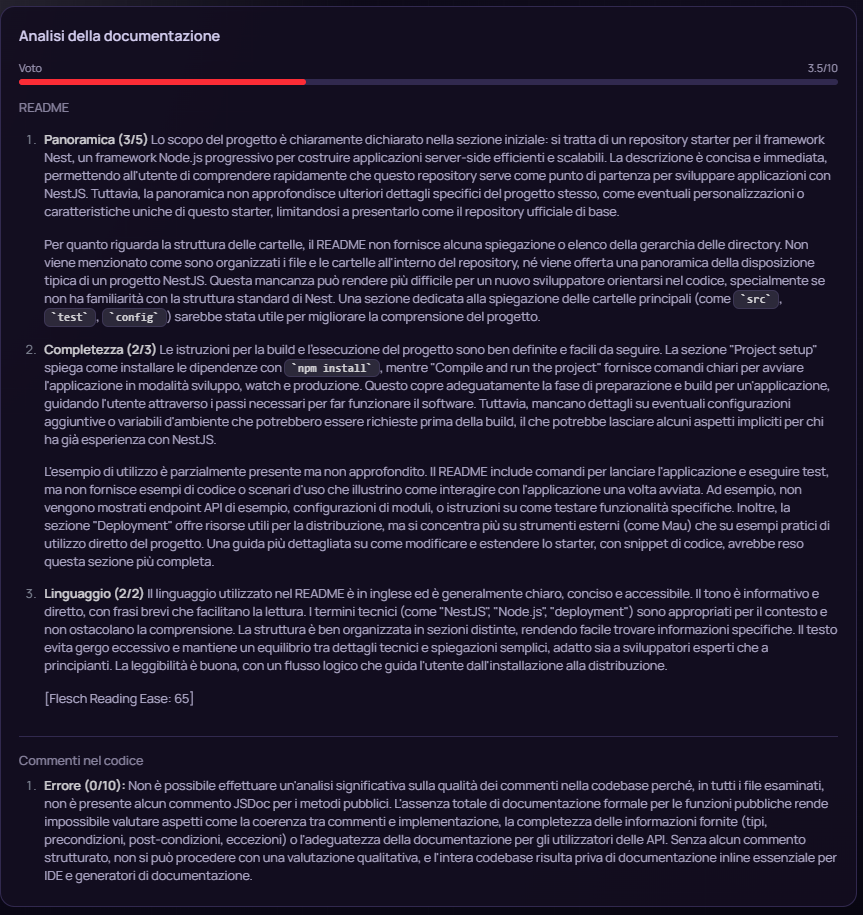
\includegraphics[width=0.8\textwidth]{../Assets/manuale_utente/SezioneDocumentazione.png}  
\caption{Sezione Documentazione}
\label{fig:report-docs}
\end{figure}

\subsection{Cambio branch e aggiornamento del report}
Cambiando la selezione nel menu \textbf{Branch}, il report mostrato si aggiorna automaticamente al contenuto dell'ultima scansione di quel branch. Se il branch non è mai stato scansionato, viene mostrato il messaggio «\textit{Nessun report disponibile per questo branch}».

% =====================================================================
\section{Risoluzione dei problemi}
% =====================================================================

\subsection{Problemi generali}

\rowcolors{2}{LightGray}{white}
\begin{longtable}{>{\raggedright\arraybackslash}p{5cm} >{\raggedright\arraybackslash}p{9cm}}
  \rowcolor{AccentColor}
  \textcolor{white}{\textbf{Problema}} &
  \textcolor{white}{\textbf{Soluzione}} \\
  \endfirsthead

  \rowcolor{AccentColor}
  \textcolor{white}{\textbf{Problema}} &
  \textcolor{white}{\textbf{Soluzione}} \\
  \endhead

  La pagina appare non formattata o con stili corrotti &
  Pulire la cache del browser e ricaricare la pagina. Verificare inoltre che il browser in uso rispetti i requisiti minimi (tabella~\ref{tab:browser}). \\
  Alcuni pulsanti non rispondono al click &
  Può essere in corso un'operazione asincrona. Attendere qualche secondo; se il problema persiste, ricaricare la pagina. \\
  La modalità scura non viene mantenuta fra le sessioni &
  Verificare di aver abilitato la memorizzazione locale (LocalStorage) per il sito. Alcune configurazioni di privacy del browser la disabilitano. \\
  Errore generico «Errore HTTP 500» &
  Problema lato server. Riprovare più tardi; se il problema persiste, segnalarlo all'amministratore includendo data, ora e azione che lo ha causato. \\
\caption{Problemi generali}
\label{tab:problemi-generali}
\end{longtable}


\subsection{Problemi di autenticazione}
Si veda la tabella riportata nella sezione~\ref{sec:errori-login}.

\subsection{Problemi con i repository GitHub}

\rowcolors{2}{LightGray}{white}
\begin{longtable}{>{\raggedright\arraybackslash}p{5cm} >{\raggedright\arraybackslash}p{9cm}}
  \rowcolor{AccentColor}
  \textcolor{white}{\textbf{Problema}} &
  \textcolor{white}{\textbf{Soluzione}} \\
  \endfirsthead

  \rowcolor{AccentColor}
  \textcolor{white}{\textbf{Problema}} &
  \textcolor{white}{\textbf{Soluzione}} \\
  \endhead

  Non riesco ad aggiungere un repository privato &
  Verificare di aver fornito un Personal Access Token valido con scope \texttt{repo}. Il token deve essere di proprietà di un utente GitHub che ha accesso al repository. \\
  Il token è stato revocato da GitHub &
  Generare un nuovo token e aggiornarlo seguendo la procedura della sezione~\ref{sec:token}. \\
  La lista dei branch è vuota &
  Il token non ha i permessi necessari, oppure il repository è stato reso privato dopo essere stato aggiunto. Aggiornare il token. \\
  Il repository GitHub è stato cancellato &
  Il repository non potrà più essere analizzato. Rimuoverlo dal workspace. \\
\caption{Problemi con i repository GitHub}
\label{tab:problemi-repo}
\end{longtable}

\subsection{Problemi con le scansioni}
Si veda anche la tabella dedicata nella sezione relativa alla scansione (tabella~\ref{tab:errori-scan}).

\rowcolors{2}{LightGray}{white}
\begin{longtable}{>{\raggedright\arraybackslash}p{5cm} >{\raggedright\arraybackslash}p{9cm}}
  \rowcolor{AccentColor}
  \textcolor{white}{\textbf{Problema}} &
  \textcolor{white}{\textbf{Soluzione}} \\
  \endfirsthead

  \rowcolor{AccentColor}
  \textcolor{white}{\textbf{Problema}} &
  \textcolor{white}{\textbf{Soluzione}} \\
  \endhead

  La scansione fallisce sempre sullo stesso branch &
  Verificare che il branch esista ancora su GitHub. Se il repository è privato, verificare che il token sia ancora valido. \\
  Il voto di sicurezza è 0 ma non ci sono vulnerabilità &
  Potrebbe trattarsi di una scansione non completata correttamente. Rilanciare la scansione. \\
  Il report non contiene la sezione «Riepilogo» &
  La sezione è opzionale: non viene mostrata se l'agente non ha generato un riepilogo testuale. \\
\caption{Problemi con le scansioni}
\label{tab:problemi-scan}
\end{longtable}

% =====================================================================
\section{Glossario}\label{sec:glossario}
% =====================================================================

I termini di seguito riportati sono contrassegnati con la lettera «G» in apice lungo l'intero documento.

\subsection{Agente}
Programma software basato su intelligenza artificiale in grado di interagire con il proprio ambiente, raccogliere dati ed eseguire attività autodirette per raggiungere un obiettivo prestabilito. In CodeGuardian gli agenti si occupano di analizzare test, documentazione e sicurezza di un repository.

\subsection{Amazon Cognito}
Servizio AWS che gestisce l'autenticazione degli utenti di CodeGuardian, fornendo il login unico tramite flusso OAuth 2.0.

\subsection{AWS}
Amazon Web Services: insieme di servizi di cloud computing offerti da Amazon. CodeGuardian utilizza diversi servizi AWS per il deployment e l'autenticazione.

\subsection{Branch}
Linea di sviluppo indipendente all'interno di un repository Git. In CodeGuardian ogni scansione è eseguita su uno specifico branch e genera un report dedicato.

\subsection{Commit}
Operazione tramite la quale le modifiche apportate ai file vengono salvate in modo definitivo all'interno di un repository. Costituisce un'istantanea dello stato del progetto in un preciso momento.

\subsection{CVE}
Common Vulnerabilities and Exposures: identificativo univoco di una vulnerabilità di sicurezza nota pubblicamente. CodeGuardian riferisce le vulnerabilità nelle dipendenze tramite il relativo CVE.

\subsection{CWE}
Common Weakness Enumeration: catalogo standard delle categorie di debolezza del software. A ogni vulnerabilità nel codice rilevata da CodeGuardian può essere associato un codice CWE.

\subsection{Developer}
Ruolo utente di CodeGuardian dedicato a chi consulta i repository e i report per applicare le correzioni suggerite. Ha permessi operativi (avvio scansioni, consultazione report) ma non amministrativi.

\subsection{Documentazione}
Insieme dei file di testo, manuali e commenti presenti in un repository che descrivono il funzionamento, la struttura e le modalità d'uso del software. In CodeGuardian un agente dedicato valuta chiarezza e completezza della documentazione.

\subsection{GitHub}
Servizio di hosting per progetti software basato su Git. Permette il versionamento online dei file e la collaborazione fra più utenti. CodeGuardian analizza i repository ospitati su GitHub.

\subsection{Membership}
Associazione fra un utente e un workspace, corredata da un ruolo (project manager, tech lead o developer). La membership viene creata tramite un invito accettato.

\subsection{OWASP}
Open Worldwide Application Security Project: fondazione globale senza scopo di lucro che produce articoli, metodologie e strumenti per migliorare la sicurezza del software. CodeGuardian verifica il codice rispetto alle vulnerabilità elencate nella OWASP Top 10.

\subsection{Owner}
Utente che ha creato un workspace. L'owner è l'unico che può eliminare definitivamente il workspace.

\subsection{Personal Access Token}
Token di autenticazione generato dall'utente dalle proprie impostazioni GitHub. In CodeGuardian viene utilizzato per autorizzare l'accesso in lettura ai repository privati. I formati accettati sono \texttt{ghp\_\ldots} (classic) e \texttt{github\_pat\_\ldots} (fine-grained).

\subsection{Project Manager}
Ruolo utente di CodeGuardian dedicato alla gestione complessiva del workspace: aggiunta e rimozione membri, gestione repository, supervisione delle attività.

\subsection{Report}
Documento generato dagli agenti di CodeGuardian al termine di una scansione, che raccoglie le valutazioni su tecnologie, test, sicurezza e documentazione, insieme a suggerimenti per il miglioramento.

\subsection{Repository}
Archivio digitale utilizzato per memorizzare, gestire e organizzare dati, codice sorgente e documenti. I repository GitHub possono avere più collaboratori e tracciano la storia di tutti i cambiamenti ai file. Abbreviato in «repo».

\subsection{Scansione}
Esecuzione di una singola analisi da parte degli agenti su uno specifico branch di un repository. Una scansione può essere in corso, completata, interrotta o terminata con errore.

\subsection{Sessione}
Intervallo di tempo durante il quale l'utente risulta autenticato. La sessione ha durata limitata e viene gestita tramite i token forniti da Cognito.

\subsection{Tech Lead}
Ruolo utente di CodeGuardian dedicato al coordinamento tecnico: aggiunta e configurazione dei repository, gestione dei token, avvio delle scansioni.

\subsection{Workspace}
Contenitore collaborativo di CodeGuardian in cui più utenti condividono repository e report. Ogni workspace ha un owner, zero o più membri e un insieme di repository associati.

\end{document}